\documentclass[]{elsarticle} %review=doublespace preprint=single 5p=2 column
%%% Begin My package additions %%%%%%%%%%%%%%%%%%%
\usepackage[hyphens]{url}



\usepackage{lineno} % add
\providecommand{\tightlist}{%
  \setlength{\itemsep}{0pt}\setlength{\parskip}{0pt}}

\usepackage{graphicx}
\usepackage{booktabs} % book-quality tables
%%%%%%%%%%%%%%%% end my additions to header

\usepackage[T1]{fontenc}
\usepackage{lmodern}
\usepackage{amssymb,amsmath}
\usepackage{ifxetex,ifluatex}
\usepackage{fixltx2e} % provides \textsubscript
% use upquote if available, for straight quotes in verbatim environments
\IfFileExists{upquote.sty}{\usepackage{upquote}}{}
\ifnum 0\ifxetex 1\fi\ifluatex 1\fi=0 % if pdftex
  \usepackage[utf8]{inputenc}
\else % if luatex or xelatex
  \usepackage{fontspec}
  \ifxetex
    \usepackage{xltxtra,xunicode}
  \fi
  \defaultfontfeatures{Mapping=tex-text,Scale=MatchLowercase}
  \newcommand{\euro}{€}
\fi
% use microtype if available
\IfFileExists{microtype.sty}{\usepackage{microtype}}{}
\bibliographystyle{elsarticle-harv}
\ifxetex
  \usepackage[setpagesize=false, % page size defined by xetex
              unicode=false, % unicode breaks when used with xetex
              xetex]{hyperref}
\else
  \usepackage[unicode=true]{hyperref}
\fi
\hypersetup{breaklinks=true,
            bookmarks=true,
            pdfauthor={},
            pdftitle={A Short Example - Canadian Behaviours for the Design of Electric Vehicle Powertrain Combinations},
            colorlinks=false,
            urlcolor=blue,
            linkcolor=magenta,
            pdfborder={0 0 0}}
\urlstyle{same}  % don't use monospace font for urls

\setcounter{secnumdepth}{5}
% Pandoc toggle for numbering sections (defaults to be off)
% Pandoc header
\usepackage{float}
\usepackage{graphicx}



\begin{document}
\begin{frontmatter}

  \title{A Short Example - Canadian Behaviours for the Design of Electric Vehicle
Powertrain Combinations}
    \author[McMaster Institute for Transportation and Logistics]{Sean Sears\corref{c1}}
   \ead{searssl@mcmaster.ca} 
   \cortext[c1]{Corresponding Author}
      \address[McMaster Institute for Transportation and Logistics]{McMaster Institute for Transportation and Logistics, School of Geography
and Earth Sciences, 1280 Main Street West, Hamilton, Ontario, L8S 4L8}
  
  \begin{abstract}
  This paper is a very short demonstration of consumer attitudes towards
  EV powertrain and body type combinations in Canada. There is a focus on
  the impact of incentives and the modelling of purchase price, operating
  cost, incentive, and vehicle age importance in vehicle purchasing
  decisions. Additionally, powertrain combinations are compared against
  survey questions to provide a sense of whether underlying biases or
  concerns impact how consumers may design vehicles, even in realistic but
  hypothetical scenarios.
  \end{abstract}
  
 \end{frontmatter}

\section{Introduction}\label{introduction}

The transportation sector represents one of the single largest
contributors to greenhouse gas emissions (GHGs) and other pollutants in
Canada. The uptake of electric vehicles (EVs), to date, has been
limited. Various authors have explored attitudes towards EVs and have
generally found purchase cost, range anxiety, and battery
maintainability to be the primary barriers to purchase (see Mohamed
(2018)). In this paper, as a part of the \emph{McMaster Institute for
Transportation and Logistic's} study on \emph{The Social Costs and
Benefits of Electric Mobility in Canada}, we aim to understand how
consumers would design and purchase a vehicle of their preferred body
type (sub-compact, Luxury Sedan, SUV, etc.) at a realistic price point.
This paper presents a small number of results from the survey itself in
addition to some basic discrete choice modeling, looking at the impact
of purchase, price, operating cost, incentives, and body types. First,
we will review the data collection process and aspects of the collection
instrument, then present the data analysis, followed by some of the
survey results and how the vehilces designed compare, lastly some
conclusions are drawn.

\section{Data Collection}\label{data-collection}

Data was collected via an electronic survey completed by a third-party
firm. A total of \textasciitilde{}20,000 observations were collected,
including repeat respondents from a version of the survey conducted in
2015. A total of 16,901 respondents are included in this analysis
dataset after removing repeat respondents and other responses inline
with other works that have used this dataset as their basis. While other
works focus on the results of the full survey (reference, reference,
mitl report), this analysis looks at the experimental section added for
the 2018 iteration of the survey, referred to as the \emph{Vehicle
Design Scenarios} (VDS).

\begin{figure}

{\centering 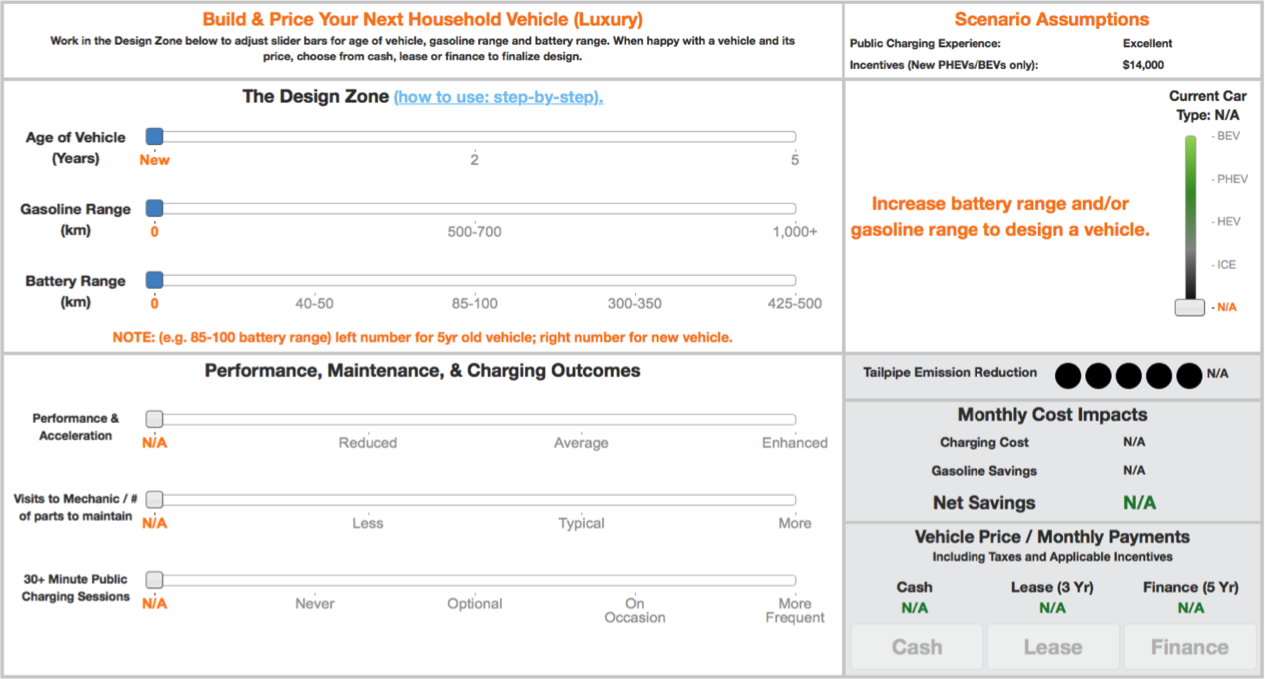
\includegraphics[width=1\linewidth]{figures/VDS_Init} 

}

\caption{\label{fig:VDS-Int} Initalized Vehicle Design Scenario}\label{fig:fig-VDS-Int}
\end{figure}

Respondents were asked to go through two VDSs where they would choose a
set of powertrain features (gasoline and electric range) that produce a
vehicle, at a price, they would be willing to purchase. It is worth
noting that as a part of the respondent screening process, only
responses that had some degree of intention of purchasing a vehicle in
the near future (as opposed to zero intent) were asked to complete the
survey. In each of the two scenarios, respondents where given a number
of assumptions to respond to, including: the ease or challenge they
could charge their EVs (Charging stations being nearby, no wait time to
plug in, and fast charging times - or not), a range of government cash
incentives applied to the purchase price (\$0, \$7000, and \$14000), and
whether or not respondents would be able to readily charge their
vehicles at home with minimal need for public charging otherwise. These
assumptions could not be changed by the respondent.

Inside of the VDS respondents, were able to assess how the performance,
maintainability, and charging outcomes of the vehicle designed would
change as the age, gasoline range, and electric range values were
changed to create different configurations. Additionally, respondents
were given information on the tailpipe emissions, in respect to a
standard internal combustion engine, information on the estimated cost
to charge their vehicle (based on the capacity of existing battery
technology and their specified annual kilometres driven), and how much
they may, potentially save on gasoline. The final piece of information
given is an approximation of the vehicle purchase price (based off of
existing vehicles and black book values are used to estimate the value
of used vehicle prices), after tax and incentives, which is also
presented as lease and financing payments. The standard initialization
of the VDS, Figure \ref{fig:VDS-Int}, begins with all sliders set to
zero values. Respondents are able to adjust the age and range sliders as
many times as they perceived necessary, but are required to move either
the gasoline or electric range sliders at least once to complete a
vehicle configuration and choose a payment method to proceed. Once a
configuration has been selected, Figure \ref{fig:VDS-Sel}, the
aforementioned fields are populated and adjust in real-time as the
respondent alters their configuration.

\begin{figure}

{\centering 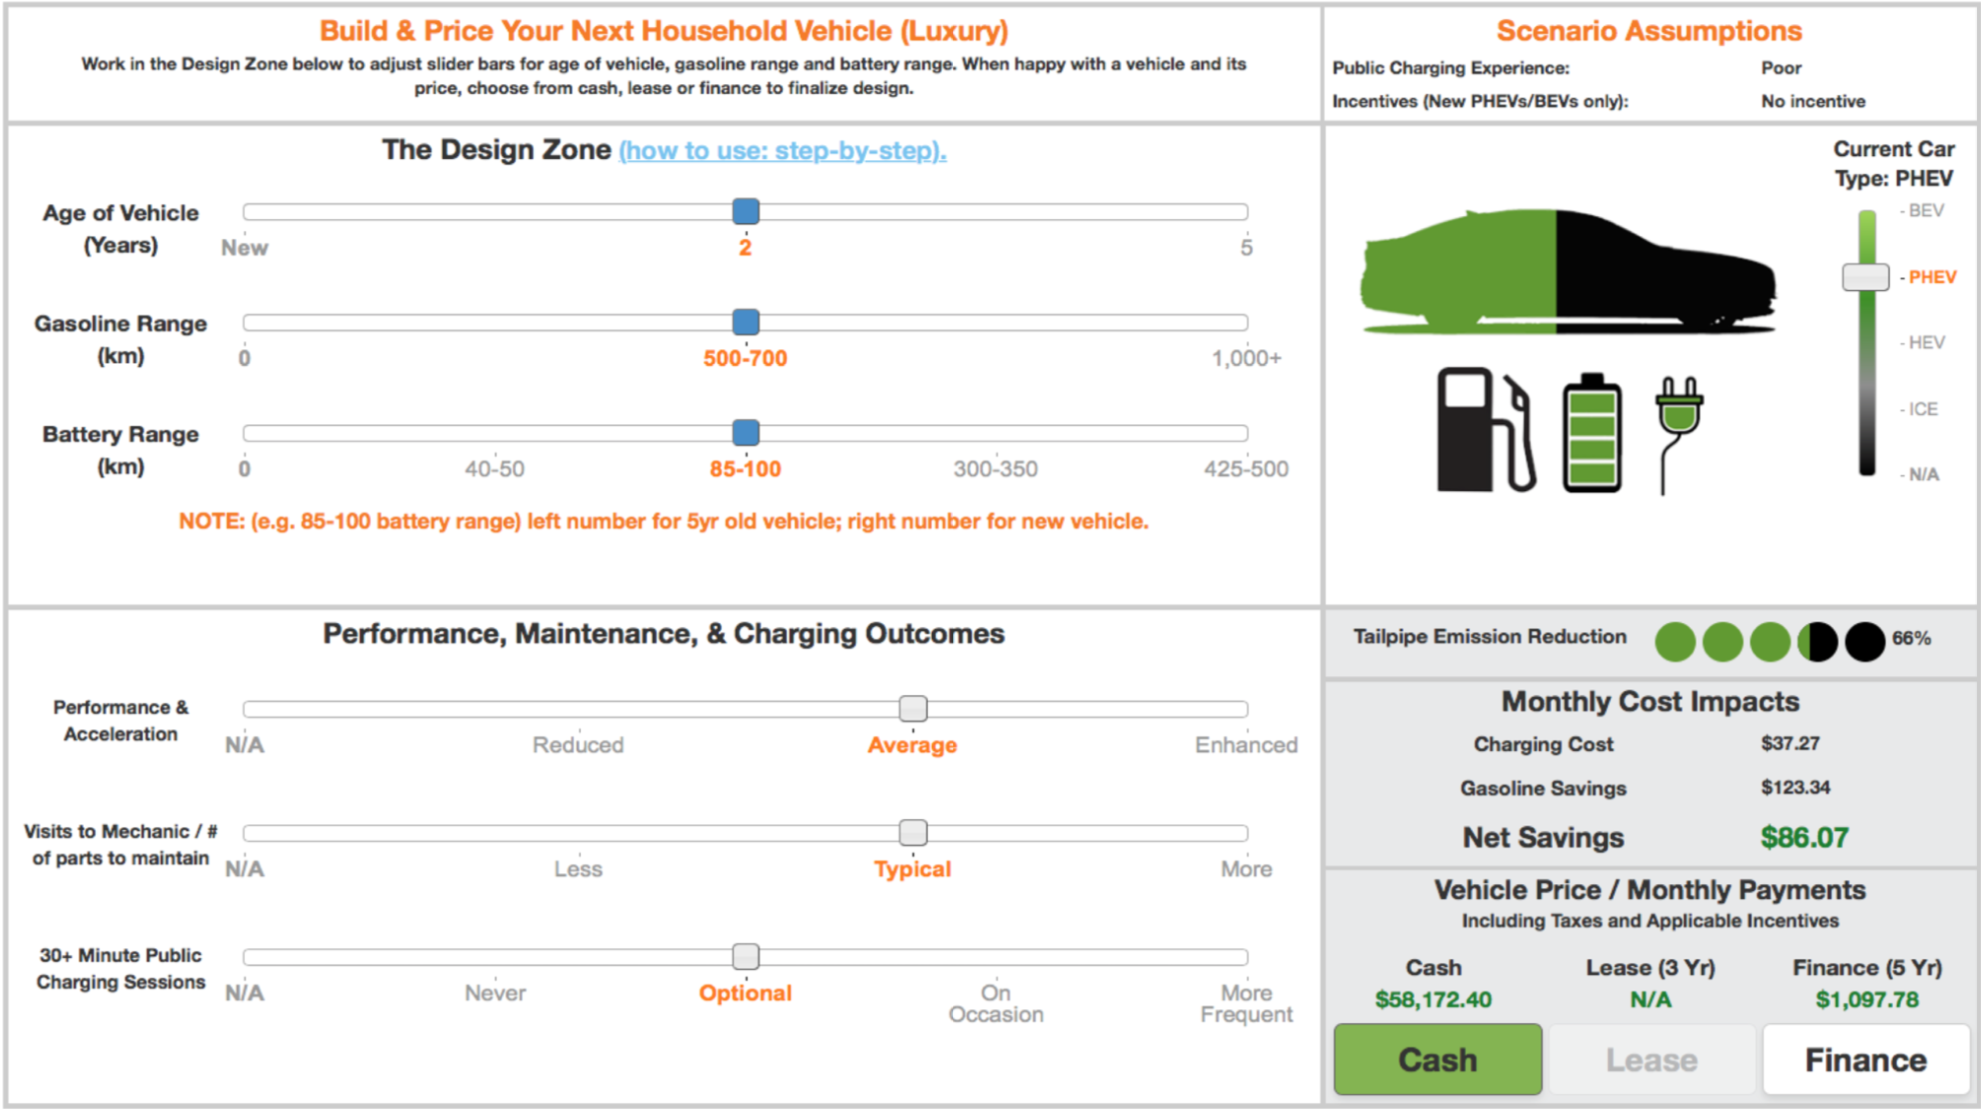
\includegraphics[width=1\linewidth]{figures/VDS_Selected} 

}

\caption{\label{fig:VDS-Sel}Vehicle Design Scenario with Configuration}\label{fig:fig-VDS-Sel}
\end{figure}

\section{Data Analysis}\label{data-analysis}

After cleaning the data of bad responses, as defined by too few slider
changes (less than 1) in the VDS or completeing the VDS too fast or too
slowly (+- 3 standard deviations of the mean), we analyze the 16, 758
remaining responses. As discussed above, respondents were asked about
the type of vehicle they would be interested in purchasing in the
future, in addition to their annual kilometerage. These values were used
to influence the purchase price of the vehicle (which varys by the body
type and the powertrain) and informed the operating cost calculation
(which estimates the monthly cost to operate the vehicle based on how
far the respondent drives), discussed in detail in Appendix 1.

\begin{table}[t]

\caption{\label{tab:prop}Purchase Price, Operating Cost, and Proprotion of Vehicles Designed}
\centering
\begin{tabular}{cccccc}
\toprule
\multicolumn{1}{c}{Vehicle Powertrain} & \multicolumn{2}{c}{Purchase Price˜ (\$)} & \multicolumn{2}{c}{Operating Cost* (\$)} & \multicolumn{1}{c}{Proportion (\%)} \\
\cmidrule(l{3pt}r{3pt}){1-1} \cmidrule(l{3pt}r{3pt}){2-3} \cmidrule(l{3pt}r{3pt}){4-5} \cmidrule(l{3pt}r{3pt}){6-6}
 & Mean & Median & Mean & Median & As Selected\\
\midrule
\addlinespace[0.3em]
\multicolumn{6}{l}{\textbf{Gasoline Only}}\\
\hspace{1em}ICE & 26163.31 & 23730.00 & 97.06 & 96.53 & 18.20\\
\hspace{1em}HEV & 41579.87 & 37070.00 & 55.65 & 55.34 & 2.78\\
\addlinespace[0.3em]
\multicolumn{6}{l}{\textbf{Gasoline \& Electricity}}\\
\hspace{1em}PHEV SE & 36084.92 & 33933.90 & 71.41 & 70.73 & 13.00\\
\hspace{1em}PHEV LE & 39960.16 & 38321.74 & 62.71 & 65.12 & 53.65\\
\hspace{1em}PHEV LG & 34113.51 & 29290.00 & 50.25 & 50.24 & 2.63\\
\addlinespace[0.3em]
\multicolumn{6}{l}{\textbf{Electricity Only}}\\
\hspace{1em}BEV SE & 32653.75 & 26530.43 & 33.14 & 34.31 & 5.74\\
\hspace{1em}BEV LE & 31007.28 & 25764.00 & 32.49 & 31.15 & 4.01\\
\bottomrule
\multicolumn{6}{l}{\textit{Note: }}\\
\multicolumn{6}{l}{˜ Approximate cost to purchase a class-represntative vehicle, inclusive of tax}\\
\multicolumn{6}{l}{* Approximate cost to operate (drive) a class-representative vehicle for 1,000km}\\
\end{tabular}
\end{table}

\subsection{Initial Outcomes}\label{initial-outcomes}

The purchase price and operating cost of vehicles, in addition to the
percentage of vehicles designed by powertrain designation, is reviewed
in Table\ref{tab:prop}. Of particular interest is the popularity of the
long-electric range plug-in hybrid electric powertrain, with 53.65\% of
respondents \emph{designing} this option. The ICE and PHEV
short-electric round out the top three selections, with the remaining
powertrains accounting for only 15\% of designs. Predicted to be of
great influence is how the operating cost was presented to respondents;
rather than in ambigous terms of per-so-many-kilometres, a clear cut
monthly dollar value was defined. The PHEV long-electric is not the
cheapest vehicle to purchase, and is actually considerably more
expensive than the most of the other powertrain combinations. This is a
curious result which will require further validation and testing. Of
concerns noted, is that for respondents who were fatigued at this stage
of the data collection (the VDS was towards the end), only moving the
sliders once or twice may have been enough for them and were not
interested in vesting the time to generate a more reflective response.
Further data cleaning could be enacted to review this phenomena, which
further consideration of the time spent and changes made variables. The
variance in vehicle purchase price by body type and powertrain is shown
in Figure \ref{fig-boxplotPP} and the variance in purchase price by
powertrain, incentive, and vehicle age is shown in Figure
\ref{fig-boxplot-PP-InctAge}. The boxplots clearly demonstrate that
vehicle purchase price decreases for new vehicles with the incentive
levels, but notably incentives do not impact the value of used vehicles.
Rather, the purchase prices fall due to depreciation. The VDS took into
active consideration the relative cost of different vehicle body types
and has integrated these variances into the experiment, as presented.

Exploring the data of the boxplots more with more depth, we look at
Table \ref{tab:prop2} for the breakdown by incentive, age, and
powertrain. A surprisingly result is how marginal the variations between
incentive groups are in the proportion of vehicles designed. While this
table does not break out the results to include the seven body types,
there is virtually no meaningful change as a result of increasing
incentives, seeing less than a .4\% change for the fully electric BEVs
and less than 1\% for the PHEVs at the maximum \$14 000 incentive level.

To further evaluate and analyze the data, a very brief discrete choice
model is looked at (see Train (2009)).

\begin{figure}

{\centering 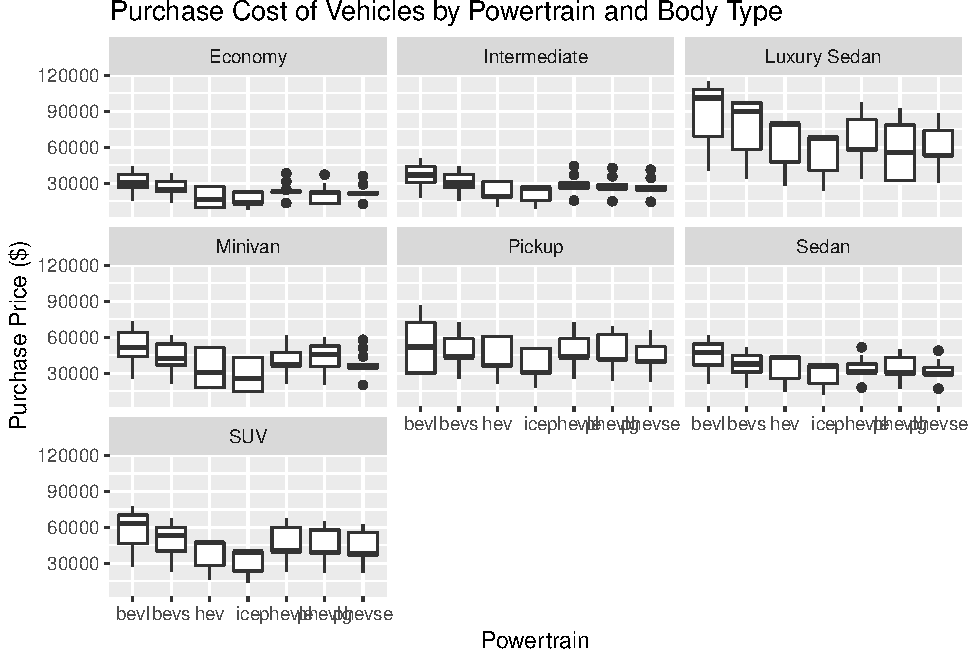
\includegraphics[width=1\linewidth]{Survey_Results_files/figure-latex/fig-boxplotPP-1} 

}

\caption{\label{fig-boxplotPP}Purchase Cost Variance by Body Type}\label{fig:fig-boxplotPP}
\end{figure}

\begin{figure}

{\centering 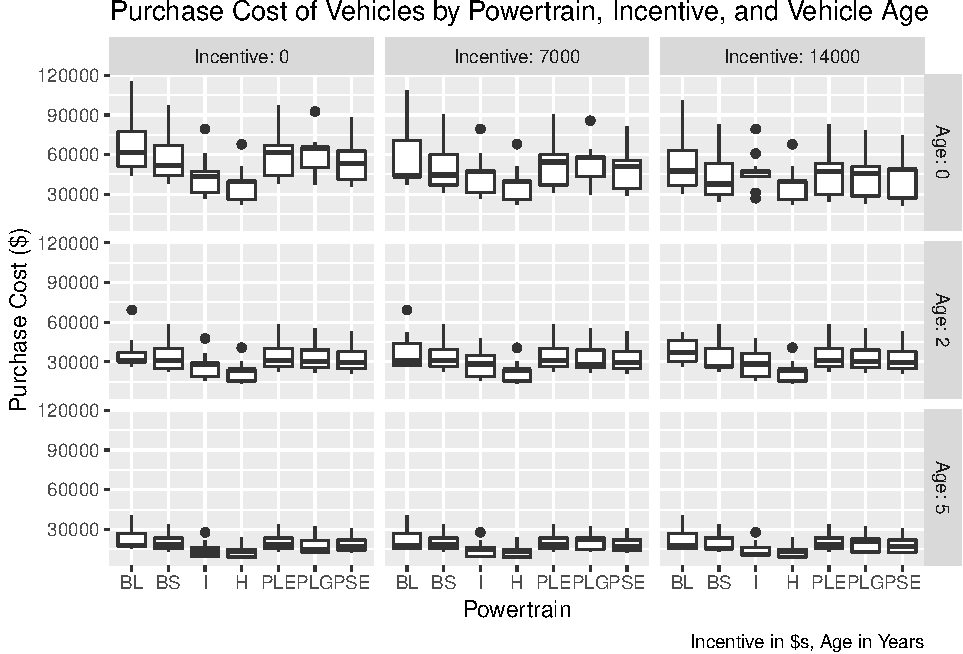
\includegraphics[width=1\linewidth]{Survey_Results_files/figure-latex/fig-boxplot-PP-InctAge-1} 

}

\caption{\label{fig-boxplot-PP-InctAge}Purchase Cost Variance by Powertrain, Incentives, and Vehicle Age}\label{fig:fig-boxplot-PP-InctAge}
\end{figure}

\begin{table}[t]

\caption{\label{tab:prop2}Mean Purchase Price of Vehicle by Powertrain, Incentive, and Vehicle Age}
\centering
\resizebox{\linewidth}{!}{
\begin{tabular}{ccccc}
\toprule
\multicolumn{1}{c}{ } & \multicolumn{3}{c}{Average Purchase Price (\$)} & \multicolumn{1}{c}{Proportion (\%)} \\
\cmidrule(l{3pt}r{3pt}){2-4} \cmidrule(l{3pt}r{3pt}){5-5}
Powertrain & New Vehicle & 2 Year Old Vehicle & 5 Year Old Vehicle & As Selected\\
\midrule
\addlinespace[0.3em]
\multicolumn{5}{l}{\textbf{\$0 Incentive}}\\
\hspace{1em}ICE & 35930.25 & 21052.50 & 12236.01 & 6.73\\
\hspace{1em}HEV & 48626.75 & 38038.00 & 27395.80 & 1.00\\
\hspace{1em}PHEV SE & 39118.97 & 39688.13 & 37737.69 & 4.47\\
\hspace{1em}PHEV LE & 47478.40 & 43207.25 & 31437.84 & 17.51\\
\hspace{1em}PHEV LG & 29966.67 & 31832.85 & 39836.52 & 0.79\\
\hspace{1em}BEV SE & 27343.83 & 39472.29 & 34484.52 & 1.74\\
\hspace{1em}BEV LE & 24239.20 & 30076.62 & 37246.88 & 1.21\\
\addlinespace[0.3em]
\multicolumn{5}{l}{\textbf{\$7 000 Incentive}}\\
\hspace{1em}ICE & 36112.58 & 20883.05 & 12280.12 & 5.87\\
\hspace{1em}HEV & 50695.07 & 38032.88 & 27143.62 & 0.92\\
\hspace{1em}PHEV SE & 32464.60 & 32476.54 & 30405.86 & 4.46\\
\hspace{1em}PHEV LE & 43317.27 & 39128.35 & 36987.74 & 17.70\\
\hspace{1em}PHEV LG & 39102.64 & 39025.98 & 34280.83 & 0.87\\
\hspace{1em}BEV SE & 40009.38 & 31832.16 & 33172.03 & 1.86\\
\hspace{1em}BEV LE & 28266.41 & 34166.15 & 34468.11 & 1.20\\
\addlinespace[0.3em]
\multicolumn{5}{l}{\textbf{\$14 000 Incentive}}\\
\hspace{1em}ICE & 35954.55 & 21141.04 & 12055.25 & 5.61\\
\hspace{1em}HEV & 50168.36 & 38034.24 & 26888.45 & 0.86\\
\hspace{1em}PHEV SE & 30856.02 & 39827.62 & 46632.97 & 4.06\\
\hspace{1em}PHEV LE & 33208.34 & 38773.15 & 34874.95 & 18.43\\
\hspace{1em}PHEV LG & 34068.44 & 33121.63 & 37770.84 & 0.97\\
\hspace{1em}BEV SE & 23492.37 & 34608.95 & 27400.65 & 2.14\\
\hspace{1em}BEV LE & 30603.00 & 36044.98 & 28650.61 & 1.60\\
\bottomrule
\end{tabular}}
\end{table}

\subsection{Estimating an Initial
Model}\label{estimating-an-initial-model}

First, a multinomial logit model will be estimated. The initial model is
estimated as \(depvar = \beta + pp\), while a second model is estimated
as \(depvar = \beta + pp + oc\). Simply the dependent variable, the
powertrain selection, is estimated to be a function of the purchase
price and the operating cost. The model output confirms (albeit from a
derived dataset), the alternatives (i.e., powertrains) frequencies. The
results, in Table \ref{tab:sadmnl}, are otherwise underwhelming. It is
not expected that the coefficients would be positive, implying that as
the values increase so too does the utility. While potentially true for
purchase price, it seems suspicious in terms of operating cost. After
the dataset has been validated, a proportional ordinal logistics
regression should be estimated in addition to mixed logit models using
the polr and gmnl packages.

\begin{table}[t]

\caption{\label{tab:sadmnl}Initial logit models}
\centering
\begin{tabular}{ccccc}
\toprule
\multicolumn{1}{c}{ } & \multicolumn{2}{c}{Initial Model} & \multicolumn{2}{c}{Second Model} \\
\cmidrule(l{3pt}r{3pt}){2-3} \cmidrule(l{3pt}r{3pt}){4-5}
Variable & Estimate & p-value & Estimate & p-value\\
\midrule
bevl:(intercept) & -1.5199 & 0.0000 & -0.7799 & 0.0000\\
bevs:(intercept) & -1.1635 & 0.0000 & -0.4323 & 0.0000\\
hev:(intercept) & -1.9016 & 0.0000 & -1.4284 & 0.0000\\
phevle:(intercept) & 1.0609 & 0.0000 & 1.4569 & 0.0000\\
phevlg:(intercept) & -1.9479 & 0.0000 & -1.4091 & 0.0000\\
\addlinespace
phevse:(intercept) & -0.3513 & 0.0000 & -0.0553 & 0.2598\\
pp & 0.0000 & 0.0117 & 0.0000 & 0.0082\\
oc & NA & NA & 0.0114 & 0.0000\\
\bottomrule
\end{tabular}
\end{table}

\section{Conclusions}\label{conclusions}

Significant time needs to be spent reflecting on the data analysis and
data capture to ensure the validity of these results. It is circumspect
that purchase price and operating cost would both be positively related,
given the expectation that as operating cost decreased the utility would
have increased. The same may be true of purchase price, but there are
more variables at play, including for some individuals, a more expensive
vehicle may in of itself be of higher utility. Other body types, such as
minivans and pickup trucks are naturally more expensive than compact
sedans. Regardless, more time is required to analyze the data to
determine the validity of the results.

\section{Acknowledgements}\label{acknowledgements}

This study is a part of a research project funded by Social Sciences and
Humanities Research Council of Canada (SSHRC) Grant No: 886-2013-0001.
The views expressed in this study are those of the authors and do not
necessarily reflect the funding authority.

\section{Appendix}\label{appendix}

\subsection{Purchase Price and Operating Cost
Calculations}\label{purchase-price-and-operating-cost-calculations}

Purchase price (pp) is determined by the bodytype (Economy,
Intermediate, Sedan, Luxury Sedan, SUV, Minivan, Pickup) and the
powertrain (i.e., technology type: ICE; Hybrid; PHEV - Short Electric,
Long Electric, Long Gas; and, BEV: Short Range, Long Range). ICE and
Hybrid are the cheapest options, respectively, across all bodytypes. pp
is affected by three age levels: New, 2, and 5 years old. New =
approximate MSRP value of the powertrain + bodytype configuration; 2 =
65\% retained value; and, 5 years = 35\% of retained value. pp is
affected by three incentive levels: \$0, \$7000, and \$14000. Offered
only to new vehicles of the powertrains: Phevse, Phevle, Phevlg, bevs,
bevl.

Operating Cost (oc) is determined by the bodytype-powertrain
combination, the cost of electricity, and the cost of gasoline (87
Octane / regular). Electricity rates are determined by whether
respondents have access to home charging or not. Those with access paid
13 cents / kWh, those without paid 26 cents / kWh to approximate the
cost of needing to use public / 3rd party charging systems. Cost of
gasoline was determined by the January 2018 average cost of gasoline
across Canada's top 20 municipalities, as per reporting by Statistics
Canada (Gas = \$1.17 per litre). This value does not vary across
alternatives. oc is calculated as a function of the average cost to
travel 1000km in a series of reference vehicles, from full tank to empty
on average combined fuel economy. This per 1000km value is then
multiplied by the midpoint of the ranges of stated annual kilometres
travelled by the respondent (e.g., 5000-10000km = 7500km), in an attempt
to approximate the actual cost to operate that specific respondent may
incur. A seperate sheet is available without the per-respondent cost
calculation.

\section*{References}\label{references}
\addcontentsline{toc}{section}{References}

\hypertarget{refs}{}
\hypertarget{ref-Mohamed2018}{}
Mohamed, F., M., 2018. What hinders adoption of the electric bus in
canadian transit? Perspectives of transit providers. Transportation
Research Part D: Transport and Environment 64, 134--149.
doi:\href{https://doi.org/10.1016/j.trd.2017.09.019}{10.1016/j.trd.2017.09.019}

\hypertarget{ref-Train2009}{}
Train, K., 2009. Discrete choice methods with simulation. Cambridge
University Press.


\end{document}


